\documentclass[10pt, twocolumn]{report}

\usepackage{color}
\usepackage[toc,page]{appendix}
\usepackage{authblk}
\usepackage{amsmath}
\usepackage{url}
\usepackage{graphicx}
\usepackage{float}
\usepackage{listings}

\definecolor{mygray}{rgb}{0.4,0.4,0.4}

\lstdefinestyle{cppStyle}{
	captionpos=b,
	numbers=left,
	% xleftmargin=8pt,
	numberstyle=\color{mygray}\ttfamily\tiny,
	numbersep=8pt,
	language=c++,
	keywordstyle=\color{blue}\tiny,
	stringstyle=\color{red}\tiny,
	commentstyle=\color{green}\tiny,
	basicstyle=\ttfamily\tiny,
	showstringspaces=false,
	breaklines,
	escapechar=|,
	columns=fullflexible,
}

\begin{document}

\title{Bubble Sort and Linear Regression with MPI}

\author[1]{Claudio Scheer}
\author[1]{Gabriell Araujo}
\affil[1]{Master's Degree in Computer Science - PUCRS}
\affil[ ]{\textit{\{claudio.scheer, grabriell.araujo\}@edu.pucrs.br}}

\maketitle

\section {General Setup}
Instead of using the LAD access provided by the professor, we ran our \textit{batch job} on one node in the Cerrado cluster. That is because we developed in C++17 and needed a newer version of GCC and OpenMPI than the one provided by LAD, and we already had a \textit{batch job} configured from previous works.

All experiments were executed three times and then the average execution time and the standard deviation were calculated. For the implementation using MPI, we used the master-slave architecture. In short, the slave asks the master for a job, the master sends the job to the slave, the slave processes the job and returns the result. The master waits for the slave's results using an asynchronous call. Finally, when all jobs are completed, the master waits for all the asynchronous results of the slaves and asks the slave to `commit suicide'\footnote{What a horrible scenario!}.

\section{Bubble Sort}
The bubble sort problem addressed here consists of sorting 1000 vectors with 2500 integers. Each slave receives a vector to sort and return the sorted vector to the master. Figure~\ref{fig:bubble-sort-time} shows the

\begin{figure}[h]
	\centering
	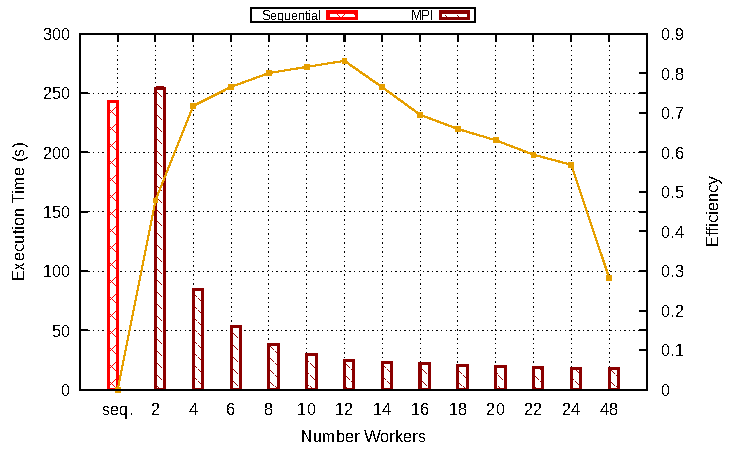
\includegraphics[width=0.45\textwidth]{../logs/scripts/bubble-sort-time.pdf}
	\caption{Execution Time x Efficiency}
	\label{fig:bubble-sort-time}
\end{figure}

\begin{figure}[h]
	\centering
	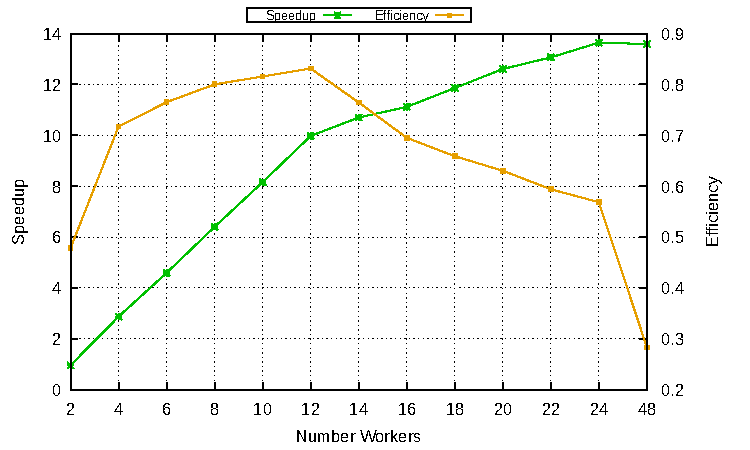
\includegraphics[width=0.45\textwidth]{../logs/scripts/bubble-sort-speedup-efficiency.pdf}
	\caption{Speedup x Efficiency}
	\label{fig:bubble-sort-speedup-efficiency}
\end{figure}

\section {Linear Regression}
Linear regression is an algorithm used for predictive analysis. In summary, the algorithm finds a relationship between $x$ and $y$ and can predict a new $y$ using as input a $x$ not yet known by the model. To test the algorithm, we used 100000000 $x$ and $y$ points.

\begin{figure}[h]
	\centering
	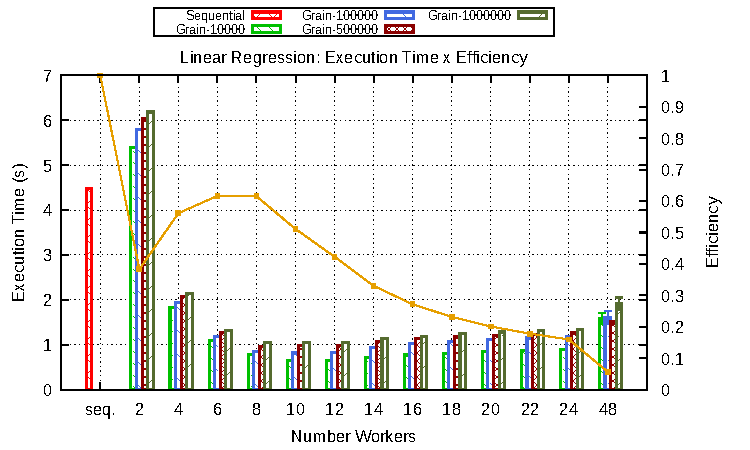
\includegraphics[width=0.45\textwidth]{../logs/scripts/linear-regression-time.pdf}
	\caption{Execution Time x Efficiency}
	\label{fig:linear-regression-time}
\end{figure}

\begin{figure}[h]
	\centering
	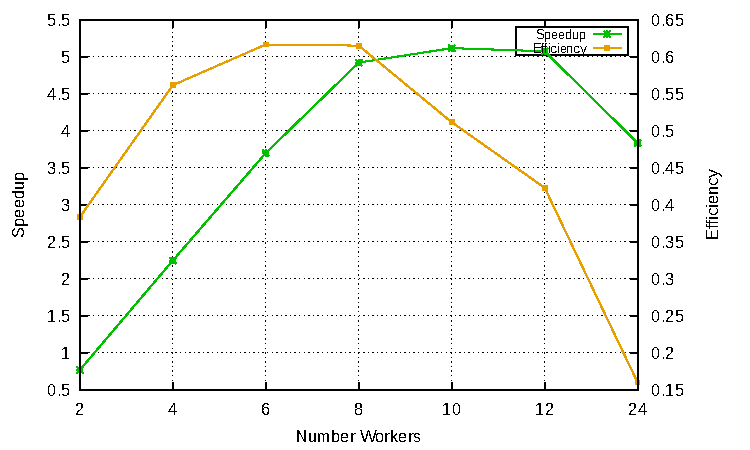
\includegraphics[width=0.45\textwidth]{../logs/scripts/linear-regression-speedup-efficiency.pdf}
	\caption{Speedup x Efficiency}
	\label{fig:linear-regression-speedup-efficiency}
\end{figure}

\section{Results}
Results of your interviews or observations. Use information and/or quotes from your interview or observations.

\begin{appendices}
	\chapter{Bubble Sort Source Code}
	\lstinputlisting[caption=Dataset generator,style=cppStyle]{../bubble-sort/dataset-generator.cpp}
	\lstinputlisting[caption=Bubble Sort Sequential,style=cppStyle]{../bubble-sort/sort-seq.cpp}
	\lstinputlisting[caption=Bubble Sort MPI,style=cppStyle]{../bubble-sort/sort-mpi.cpp}

	\chapter{Linear Regression Source Code}
	\lstinputlisting[caption=Dataset generator,style=cppStyle]{../bubble-sort/dataset-generator.cpp}
	\lstinputlisting[caption=Linear Regression Sequential,style=cppStyle]{../linear-regression/lr-seq.cpp}
	\lstinputlisting[caption=Linear Regression MPI,style=cppStyle]{../linear-regression/lr-mpi.cpp}
\end{appendices}

\end{document}
